\documentclass[12pt]{article}

\title{Sensor Fusion with Kalman Filter}
\author{Jun Zhu}
\date{\today}

\usepackage{lmodern}
\usepackage{amsmath, amsthm, amssymb, amsfonts}
\usepackage{graphicx}
\usepackage{grffile}
\usepackage{enumitem}

\usepackage{geometry}
\geometry{
	a4paper,
	left=20mm,
	right=20mm,
	top=20mm,
	bottom=20mm
}

% Define reference for color names
\usepackage[svgnames]{xcolor}
\definecolor{dodgerblue}{RGB}{30,144,255}

% Set table caption
\usepackage{caption}
\captionsetup[table]{
	skip=6pt
}

\usepackage[]{microtype}

% Set reference
\usepackage{hyperref}
\hypersetup {
	colorlinks=true,
	linkcolor=dodgerblue
}

% For fixed width table cell with alignment
\usepackage{array}
\newcolumntype{L}[1]{>{\raggedright\arraybackslash}p{#1}}
\newcolumntype{C}[1]{>{\centering\arraybackslash}p{#1}}
\newcolumntype{R}[1]{>{\raggedleft\arraybackslash}p{#1}}

% First line ident
\usepackage{indentfirst}
\setlength{\parindent}{0.75cm}


\begin{document}
\maketitle

%%%-------------------------------------------------------------------------%%%
%%%-------------------------------------------------------------------------%%%
%%%-------------------------------------------------------------------------%%%

\section{Basic Kalman Filter}\label{basic-kalman-filter}

The Kalman filter estimates a process by using a feedback control. The filter predicts the system state at some time and then obtains feedback based on measurement. The time update (prediction) function of the basic Kalman filter is governed by the linear stochastic equation
%
\begin{equation}
	\mathbf{\hat{x}}_{k} = \mathbf{F}\mathbf{\hat{x}}_{k - 1} + \mathbf{w},
\end{equation}
%
where \(\mathbf{\hat{x}}_{k} \in \mathfrak{R}^{n}\) is the estimated state vector for \(\mathbf{x_k}\) and \(\mathbf{w}\sim N( 0,\mathbf{Q})\) is the process noise with \(\mathbf{Q}\) the covariance matrix. The measurement function is written as:
%
\begin{equation}
	\mathbf{z}_{\mathbf{k}} = \mathbf{H}\mathbf{\hat{x}}_{k} + \mathbf{v},
\end{equation}
%
where \(\mathbf{z}_{k} \in \mathfrak{R}^{m}\) is the measurement vector and \(\mathbf{v}\sim N( 0,\mathbf{R})\) is the process noise with \(\mathbf{R}\) the covariance matrix.

The equations used in the Kalman filter are listed in Table~\ref{tab:table-KF} \cite{Welch}. Here \(\mathbf{P}_{k}^{-}\) and \(\mathbf{P}_{k}\) are the priori and posteriori error covariance matrix, respectively, \(\mathbf{z}_{k} - \mathbf{H}\mathbf{\hat{x}}_{k}^{-}\) is called the \textbf{\textit{measurement innovation}}, and \(\mathbf{K}_{k}\), the so-called \textbf{\textit{Kalman gain}}, is chosen to minimize the posteriori error covariance.

\begin{table}[h]
	\renewcommand{\arraystretch}{1.5}
	\caption{Discrete Kalman filter time and measurement update equations.}
	\centering
	\label{tab:table-KF}
	\begin{tabular}{C{7cm}|C{7cm}}
		\hline
		Time update (predict) & Measurement update (correct) \\
		\hline
		$\begin{aligned}[t]
			\mathbf{\hat{x}}_{k}^{-} &= \mathbf{F}\mathbf{\hat{x}}_{k - 1} \\
			\mathbf{P}_{k}^{-} &= \mathbf{F}\mathbf{P}_{k - 1}\mathbf{F}^{\mathbf{T}} + \mathbf{Q}
		\end{aligned}$ &
		$\begin{aligned}[t]
			\mathbf{K}_{k} &= \mathbf{P}_{k}^{-}\mathbf{H}^{\mathbf{T}}( \mathbf{H}\mathbf{P}_{k}^{-}\mathbf{H}^{\mathbf{T}}\mathbf{+ R})^{- 1} \\
			\mathbf{\hat{x}}_{k} &= \mathbf{\hat{x}}_{k}^{-} + \mathbf{K}_{k}( \mathbf{z}_{k} - \mathbf{H}\mathbf{\hat{x}}_{k}^{-}) \\
			\mathbf{P}_{k} &= ( \mathbf{I} - \mathbf{K}_{k}\mathbf{H})\mathbf{P}_{k}^{-}
		\end{aligned}$ \\
		\hline
	\end{tabular}
\end{table}

In the LIDAR measurement, the state vector \(\mathbf{x}\) is given by
%
\begin{equation}
	\mathbf{x} = \begin{bmatrix} p_{x} & p_{y} & \dot{p}_{x} & \dot{p}_{y}\end{bmatrix}^{T}.
\end{equation}
%
Assuming a linear motion, we have
%
\begin{equation}
	\mathbf{F} = \begin{bmatrix}
	1 & 0 & \Delta t & 0 \\
	0 & 1 & 0 & \Delta t \\
	0 & 0 & 1 & 0 \\
	0 & 0 & 0 & 1 \\
	\end{bmatrix},
\end{equation}
%
where \(\Delta t\) is the time step. The measurement vector is \(\mathbf{z}_{k} = \begin{bmatrix} p_{x} & p_{y} \end{bmatrix}^{T}\), and the measurement matrix is simply
%
\begin{equation}
	\mathbf{H} = \begin{bmatrix}
	1 & 0 & 0 & 0 \\
	0 & 1 & 0 & 0 \\
	\end{bmatrix}.
\end{equation}

%%%-------------------------------------------------------------------------%%%
%%%-------------------------------------------------------------------------%%%
%%%-------------------------------------------------------------------------%%%

\section{Extended Kalman filter}\label{extended-kalman-filter}

The extended Kalman filter is used to solve the problem in which the state function
%
\begin{equation}
	\mathbf{\hat{x}}_{k} = \mathbf{f}( \mathbf{\hat{x}}_{k - 1},\ \mathbf{w}_{k - 1})
\end{equation}
and/or the measurement function
%
\begin{equation}
	\mathbf{z}_{k} = \mathbf{h}( \mathbf{\hat{x}}_{k},\mathbf{v}_{k}).
\end{equation}
%
are nonlinear.

The equations used in the extended Kalman filter are summarized in Table 2 \cite{Welch}. Here, \(\mathbf{F}\) is the Jacobian matrix of partial derivatives of \(\mathbf{f}\) with respect to \(\mathbf{x}\), which gives
%
\begin{equation}
	F_{i,j} = \frac{\partial f_{i}}{\partial x_{j}}.
\end{equation}
%
\(\mathbf{W}\) is the Jacobian matrix of partial derivatives of \(\mathbf{f}\) with respect to \(\mathbf{w}\), which gives
%
\begin{equation}
	W_{i,j} = \frac{\partial f_{i}}{\partial w_{j}}.
\end{equation}
%
\(\mathbf{H}\) is the Jacobian matrix of partial derivatives of \(\mathbf{h}\) with respect to \(\mathbf{x}\), that is
%
\begin{equation}
	H_{i,j} = \frac{\partial h_{i}}{\partial x_{j}}.
\end{equation}
%
\(\mathbf{V}\) is the Jacobian matrix of partial derivatives of \(\mathbf{h}\) with respect to \(\mathbf{v}\), that is
%
\begin{equation}
	V_{i,j} = \frac{\partial h_{i}}{\partial v_{j}}.
\end{equation}
%
It must be noted that in the extended Kalman filter the noise is no
longer normal after the nonlinear transformation.

\begin{table}[h]
	\renewcommand{\arraystretch}{1.5}
	\caption{Extended Kalman filter time and measurement update equations.}
	\centering
	\label{tab:table-EKF}
	\begin{tabular}{C{7cm}|C{7cm}}
		\hline
		Time update (predict) & Measurement update (correct) \\
		\hline
		$\begin{aligned}[t]
			\mathbf{\hat{x}}_{k}^{-} &= \mathbf{f}( \mathbf{\hat{x}}_{k - 1}, \mathbf{0}) \\
			\mathbf{P}_{k}^{-} &= \mathbf{F}\mathbf{P}_{k - 1}\mathbf{F}^{\mathbf{T}}\mathbf{+}\mathbf{W}_{\mathbf{k}}\mathbf{Q}_{k-1}\mathbf{W}_{k}^{T}
		\end{aligned}$ &
		$\begin{aligned}[t]
			\mathbf{K}_{k} &= \mathbf{P}_{k}^{-}\mathbf{H}^{\mathbf{T}}( \mathbf{H}\mathbf{P}_{k}^{-}\mathbf{H}^{\mathbf{T}}\mathbf{+}\mathbf{V}_{k}\mathbf{R}_{k}\mathbf{V}_{k}^{T})^{- 1} \\
			\mathbf{\hat{x}}_{k} &= \mathbf{\hat{x}}_{k}^{-} + \mathbf{K}_{k}( \mathbf{z}_{k} - \mathbf{h}(\mathbf{\hat{x}}_{k}^{-},\mathbf{0})) \\
			\mathbf{P}_{k} &= ( \mathbf{I} - \mathbf{K}_{k}\mathbf{H})\mathbf{P}_{k}^{-}
		\end{aligned}$ \\
		\hline
	\end{tabular}
\end{table}

The RADAR measurement returns
%
\begin{equation}
	{\mathbf{z}_{\mathbf{k}} = \begin{bmatrix} \rho_{k} & \varphi_{k} & 	{\dot{\rho}}_{k} \end{bmatrix}}^{T}
\end{equation}
%
in the polar coordination system, which means the mapping from the state vector \(\mathbf{x}_{\mathbf{k}}\) to the measurement vector \(\mathbf{z}_{\mathbf{k}}\) is no longer linear. The transform equations from the Cartesian coordinate system to the polar coordinate system (\(\mathbf{h}\)) are given by
%
\begin{equation}
	\rho = \sqrt{p_x^{2} + p_y^{2}},\ \varphi = \arctan( \frac{p_y}{p_x}),\ 	\dot{\rho} = \frac{p_x \dot{p}_x + p_y \dot{p}_y}{\sqrt{p_x^{2} + p_y^{2}}}.
\end{equation}
%
The Jacobian matrix of \(\mathbf{h}\) is
%
\begin{equation}
	\renewcommand{\arraystretch}{1.5}
	\mathbf{H} = \begin{bmatrix}
	\frac{p_x}{\sqrt{p_x^{2} + p_y^{2}}} & \frac{p_y}{\sqrt{p_x^{2} + p_y^{2}}} & 0 & 0 \\
	 - \frac{p_y}{p_x^{2} + p_y^{2}} & \frac{p_x}{p_x^{2} + p_y^{2}} & 0 & 0 \\
	\frac{p_y( p_y \dot{p}_x - p_x \dot{p}_y)}{( p_x^{2} + p_y^{2})^{3/2}} & \frac{p_x( p_x \dot{p}_y - p_y \dot{p}_x)}{( p_x^{2} + p_y^{2})^{3/2}} & \frac{p_x}{\sqrt{p_x^{2} + p_y^{2}}} & \frac{p_y}{\sqrt{p_x^{2} + p_y^{2}}} \\
	\end{bmatrix}.
\end{equation}
%
Since the linear motion assumption still holds, \(\mathbf{F}\) is 
given by equation (4). Furthermore, we assume that the process and
measurement noises are both static. Therefore, \(\mathbf{W}\) and
\(\mathbf{V}\) are both identity matrices\textbf{.}

%%%-------------------------------------------------------------------------%%%
%%%-------------------------------------------------------------------------%%%
%%%-------------------------------------------------------------------------%%%

\section{Uncented Kalman filter}\label{uncented-kalman-filter}

\subsection{Uncented transform}
The uncented transform is a method for calculating the statistics of a random variable which undergoes a nonlinear transformation. Considering propagating a 1D state vector \(\mathbf{x}\) through a nonlinear function \(\mathbf{y} = \mathbf{f}(\mathbf{x})\). To calculate the statistics of \(\mathbf{f}\), we form a matrix \(\mathbf{\Sigma}\) consisting of 2$L$+1 sigma vectors \cite{Wan}
%
\begin{align} \label{eq:UK_start}
	\mathbf{\Sigma_0} &= \mathbf{\bar{x}} \\
	\mathbf{\Sigma_i} &= \mathbf{\bar{x}} + \sqrt{(\lambda + L)\mathbf{P_{x}}}, i=1,...,L \\
	\mathbf{\Sigma_i} &= \mathbf{\bar{x}} - \sqrt{(\lambda + L)\mathbf{P_{x}}}, i=L+1,...,2L
\end{align}
%
where \(\lambda = \alpha^{2}(L + \kappa) - L\) is a scaling parameter. The constant $\alpha \in (0, 1]$ determines the spread of the sigma points around \(\mathbf{\bar{x}}\). Another constant $\kappa$ is usually set to either 0 or $3 - L$.

These sigma vectors are propagated through the same nonlinear function
%
\begin{equation}
	\mathbf{\Gamma_i} = \mathbf{f}(\mathbf{\Sigma_i}), i = 0,...,2L
\end{equation}
%
The mean and covariance of \(\mathbf{\Gamma}\) are given by
%
\begin{equation}
	\mathbf{\bar{\Gamma}} = \sum_{i=0}^{2L} W^{(m)}_i \mathbf{\Gamma_i},
\end{equation}
%
and
\begin{equation}
	\mathbf{P_\Gamma} = \sum_{i=0}^{2L} W^{(c)}_i (\mathbf{\Gamma_i} - \mathbf{\bar{\Gamma}}) (\mathbf{\Gamma_i} - \mathbf{\bar{\Gamma}})^T
\end{equation}
%
where the weights $W_i$ is given by
%
\begin{equation} \label{eq:UK_end}
	\begin{cases}
		W^{(m)}_i &= \lambda / (L + \lambda) \\
		W^{(c)}_i &= \lambda / (L + \lambda) + 1 - \alpha^2 + \beta \\
		W_i^{(m)} &= W_i^{(c)} = 0.5/(L + \lambda), i=1,...,2L
	\end{cases}
	,
\end{equation}
%
where $\beta$ is related to the distribution of \(\mathbf{x}\) and $\beta=2$ for Gaussian distribution.

\subsection{Uncented Kalman filter equations}

The uncented Kalman filter (UKF) is a derivative-free alternative to the extended Kalman filter (EKF). In UKF, the augmented state vector is initialized as
%
\begin{equation}
	\mathbf{x}^a_0 = [\mathbf{x}^T_0, \mathbf{0}, \mathbf{0}]^T, 
\end{equation}
%
and the augmented covariance matrix is initialized as
%
\begin{equation} \label{eq:UK_aug}
	\mathbf{P}_0 = \begin{bmatrix}
	\mathbf{P}^a_0 & 0 & 0 \\
	0 & \mathbf{Q} & 0 \\
	0 & 0 & \mathbf{R} \\ 
	\end{bmatrix}
\end{equation}
%
The sigma matrix and augmented sigma matrix at step $k$ are denoted as \(\mathbf{\Sigma}_k^x\) and \(\mathbf{\Sigma}_k^a\), respectively.
%
- Time update (predict)
%
\begin{align}
	\mathbf{\Sigma}_k^{x-} &= \mathbf{f}( \mathbf{\Sigma}^x_{k-1}, \mathbf{\Sigma}^\text{w}_{k-1}) \label{eq:UK_pre1} \\
	\mathbf{x}_k^{-} &= \sum_{i=0}^{2L}{W_i^{(m)}\mathbf{\Sigma}^{x-}_{k,i}} 	\\		
	\mathbf{P}_{k}^{-} &= \sum_{i=0}^{2L}{W_i^{(c)}(\mathbf{\Sigma}^{x-}_{k,i} - 		\mathbf{x}_k^{-})(\mathbf{\Sigma}^{x-}_{k,i} - \mathbf{x}_k^{-})^T} \label{eq:UK_pre3} \\
	\mathbf{\Gamma}_k^- &= \mathbf{h}(\mathbf{\Sigma}_k^{x-}, \mathbf{\Sigma}^\text{v}_{k-1}) \label{eq:UK_pre4} \\ 
	\mathbf{z}_k^{-} &= \sum_{i=0}^{2L}{W_i^{(m)}\mathbf{\Gamma}^{-}_{k,i}}
\end{align}
%
- Measurement update (correct)
%
\begin{align}
	\mathbf{P}_{\mathbf{z}_k \mathbf{z}_k} &= \sum_{i=0}^{2L}{W_i^{(c)}(\mathbf{\Gamma}^{-}_{k,i} - \mathbf{z}_k^{-})(\mathbf{\Gamma}^{-}_{k,i} - \mathbf{z}_k^{-})^T} \label{eq:UK_cor1} \\
	\mathbf{P}_{\mathbf{x}_k \mathbf{z}_k} &= \sum_{i=0}^{2L}{W_i^{(c)}(\mathbf{\Gamma}^{-}_{k,i} - 		\mathbf{z}_k^{-})(\mathbf{\Sigma}^{x-}_{k,i} - \mathbf{x}_k^{-})^T} \\
	\mathbf{K_k} &= \mathbf{P}_{\mathbf{x}_k \mathbf{z}_k}\mathbf{P}_{\mathbf{z}_k \mathbf{z}_k}^{-1} \\
	\mathbf{x}_{k} &= \mathbf{x}_{k}^{-} + \mathbf{K}_{k}( \mathbf{z}_k - \mathbf{z}^-_k) \\
	\mathbf{P}_k &= \mathbf{P}_{k-1} - K_k\mathbf{P}_{\mathbf{z}_k \mathbf{z}_k}K_k^T
\end{align}

In the case where the process noise are purely addictive, the process noise \(\mathbf{Q}\) should be removed from the augmentation equation \ref{eq:UK_aug}, and equation \ref{eq:UK_pre1} and \ref{eq:UK_pre3} become
\begin{equation}
	\mathbf{\Sigma}_k^{x-} = \mathbf{f}( \mathbf{\Sigma}^x_{k-1})
\end{equation}
and
\begin{equation}
	\mathbf{P}_{k}^{-} = \sum_{i=0}^{2L}{W_i^{(m)}(\mathbf{\Sigma}^{x-}_{k,i} - 		\mathbf{x}_k^{-})(\mathbf{\Sigma}^{x-}_{k,i} - \mathbf{x}_k^{-})^T} + \mathbf{Q} ,
\end{equation}
respectively.

In the case where the measurement noise are purely addictive, the measurement noise \(\mathbf{Q}\) should be removed from the augmentation equation \ref{eq:UK_aug}, and equation \ref{eq:UK_pre4} and \ref{eq:UK_cor1} become
\begin{equation} \label{eq:UKF_mea_add0}
	\mathbf{\Gamma}_k^- = \mathbf{h}(\mathbf{\Sigma}_k^{x-})
\end{equation}
and
\begin{equation} \label{eq:UKF_mea_add1}
	\mathbf{P}_{\mathbf{z}_k \mathbf{z}_k} = \sum_{i=0}^{2L}{W_i^{(c)}(\mathbf{\Gamma}^{-}_{k,i} - \mathbf{z}_k^{-})(\mathbf{\Gamma}^{-}_{k,i} - \mathbf{z}_k^{-})^T} + \mathbf{R},
\end{equation}
respectively.

\subsection{UKF in CTRV model}

\subsubsection{The CTRV (Constant Turn Rate and Velocity) model}

The state vector and the velocity vector are given by
\begin{equation}
	\mathbf{x} = \begin{bmatrix}p_x & p_y & v & \psi & \dot{\psi}\end{bmatrix}^T 
\end{equation}
%
and
%
\begin{equation}
	\mathbf{v} = \begin{bmatrix}\dot{p}_x & \dot{p}_y & \dot{v} & \dot{\psi} & \ddot{\psi}\end{bmatrix}^T, 
\end{equation}
%
respectively. Since the CTRV model is use, we have $\dot{v}=0$ and $\ddot{\psi}=0$.

\begin{figure}[h]
	\center
	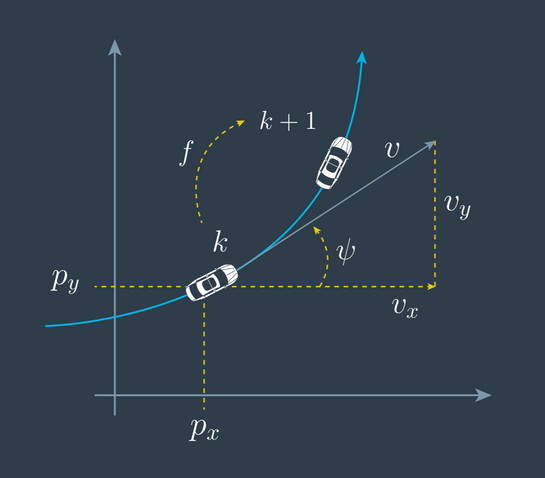
\includegraphics[scale=0.5]{./misc/CTRV_model.png}
	\caption{Illustration of the CTRV model}
	\label{fig:ctrv}
\end{figure}

The time update function can be written as
\begin{equation}
	\mathbf{x}_{k} = 
	\mathbf{x}_{k-1} + \int_{t_{k-1}}^{t_k} {\mathbf{v_{k-1}}dt} 
	= \mathbf{x}_{k-1} + 
	\begin{bmatrix} 
		v_{k-1}\int_{t_{k-1}}^{t_k} cos(\psi_{k-1}(t))dt \\
		v_{k-1}\int_{t_{k-1}}^{t_k} sin(\psi_{k-1}(t)) dt \\ 
		0 \\ 
		\dot{\psi}\Delta t \\ 
		0 
	\end{bmatrix} +
	\begin{bmatrix} \frac{1}{2}w_a\Delta t^2cos(\psi_{k-1}(t)) \\
	                \frac{1}{2}w_a\Delta t^2sin(\psi_{k-1}(t)) \\
	                \text{w}_a\Delta t \\
	                \text{w}_{\ddot{\phi}} \Delta t \\
	                0
	                \end{bmatrix}
\end{equation}
%
where
%
\begin{equation}
	v_{k-1}\int_{t_{k-1}}^{t_k} cos(\psi_{k-1}(t)) dt =
	\begin{cases}
	  v_{k-1}(sin(\psi_k) - sin(\psi_{k-1}))/\dot{\psi}_{k-1}, & \psi_{k-1} \neq 0 \\
	  v_{k-1}cos(\psi_{k-1})\Delta t, &\psi_{k-1} = 0
	\end{cases}
\end{equation}
and
\begin{equation}
	v_{k-1}\int_{t_{k-1}}^{t_k} sin(\psi_{k-1}(t)) dt =
	\begin{cases}
	  v_{k-1}(cos(\psi_{k-1}) - cos(\psi_{k}))/\dot{\psi}_{k-1}, & \psi_{k-1} \neq 0 \\
	  v_{k-1}sin(\psi_{k-1})\Delta t, &\psi_{k-1} = 0
	\end{cases}.
\end{equation}
%
During the measurement update, equations \ref{eq:UKF_mea_add0} and \ref{eq:UKF_mea_add1} can be used.

%
%%%-------------------------------------------------------------------------%%%
%%%-------------------------------------------------------------------------%%%
%%%-------------------------------------------------------------------------%%%

\section{Real-time consistency tests}

The estimation errors of a state estimator (filter) based on a finite number of samples (measurements) should be consistent with their theoretical statistical properties: \cite{Shalom}

\begin{enumerate}
	\item Have mean zero (i.e., the estimates are unbiased).
	\item Have covariance matrix as calculated by the filter.
\end{enumerate}

As a result, the consistency criteria of a filter are as follows:

\begin{enumerate}[label=(\alph*)]
	\item The state errors should be acceptable as zero mean and have magnitude commensurate with the state covariance as yielded by the filter.
	\item \textbf{The innovations should also have the same property}.
	\item \textbf{The innovations should be acceptable as white}.
\end{enumerate}

The last two criteria are the only ones that can be tested in applications with real data. The first criterion, which is really the most important one, can be tested only in simulations with the \textbf{\textit{normalized estimation error squared (NEES)}}

\begin{equation}
	\epsilon_{x,k}=(\mathbf{x}_k - \mathbf{\hat{x}}_k)^{T}\mathbf{P}^{-1}_{k}(\mathbf{x}_k - \mathbf{\hat{x}}_k).
\end{equation}
where \(\mathbf{P}_k\) is the posteriori error covariance matrix. Under the hypothesis that the filter is consistent, \(\epsilon_{x,k}\) should have a \(\chi^2\) distribution with \(n\) \((n_x)\) degrees of freedom.

Criterion (b) can be tested with the \textbf{\textit{time-average normalized innovation squared (NIS)}} statistic. For the basic Kalman filter, it is given by

\begin{equation}
  \epsilon_{z,k}=(\mathbf{z}_{k} - \mathbf{H}\mathbf{x}_{k}^{-})^{\mathbf{T}}S_k^{- 1}(\mathbf{z}_{k} - \mathbf{H}\mathbf{x}_{k}^{-}).
\end{equation}
where
\begin{equation}
	S_k=\mathbf{H}  \mathbf{P}_{k}^{-}\mathbf{H}^{\mathbf{T}}\mathbf{+ R}
\end{equation}
Note that \(S_k\) also appears on the right-hand side of the equation of calculating the Kalman gain. Under the hypothesis that the filter is consistent, \(\epsilon_{z,k}\) should have a \(\chi^2\) distribution with \(m\) \((n_z)\) degrees of freedom.
%
%%%-------------------------------------------------------------------------%%%
%%%-------------------------------------------------------------------------%%%
%%%-------------------------------------------------------------------------%%%

\section{More readings}
\noindent
\url{http://home.wlu.edu/~levys/kalman_tutorial/} \\
\url{http://biorobotics.ri.cmu.edu/papers/sbp_papers/integrated3/kleeman_kalman_basics.pdf}

%%%-------------------------------------------------------------------------%%%
%%%-------------------------------------------------------------------------%%%
%%%-------------------------------------------------------------------------%%%

\begin{thebibliography}{9}

\bibitem{Welch} 
Greg Welch and Gary Bishop.
\textit{An introduction to the Kalman filter}. 
ACM, Inc. 2001.

\bibitem{Wan} 
Eric A. Wan and Rudolph van der Merwe, 
\textit{Kalman filtering and neural networks}. p.221, John Wiley \& Sons, Inc., 2002.

\bibitem{Shalom}
Yaakov Bar-Shalom, X. Rong Li, Thiagalingam Kirubarajan,
\textit{Estimation with Applications to Tracking and Navigation: Theory, Algorithms and Software}. John Wiley \& Sons, Inc., 2001.



\end{thebibliography}


\end{document}